%File: formatting-instruction.tex
\documentclass[letterpaper]{article}
\usepackage{aaai24}
\usepackage{times}  % DO NOT CHANGE THIS
\usepackage{helvet}  % DO NOT CHANGE THIS
\usepackage{courier}  % DO NOT CHANGE THIS
\usepackage[hyphens]{url}  % DO NOT CHANGE THIS
\usepackage{graphicx} % DO NOT CHANGE THIS
\urlstyle{rm} % DO NOT CHANGE THIS
\def\UrlFont{\rm}  % DO NOT CHANGE THIS
\usepackage{natbib}  % DO NOT CHANGE THIS AND DO NOT ADD ANY OPTIONS TO IT
\usepackage{caption} % DO NOT CHANGE THIS AND DO NOT ADD ANY OPTIONS TO IT
\frenchspacing  % DO NOT CHANGE THIS
\setlength{\pdfpagewidth}{8.5in} % DO NOT CHANGE THIS
\setlength{\pdfpageheight}{11in} % DO NOT CHANGE THIS
%
% These are recommended to typeset algorithms but not required. See the subsubsection on algorithms. Remove them if you don't have algorithms in your paper.
\usepackage{algorithm}
\usepackage{algorithmic}

\makeatletter
\newcommand{\rmnum}[1]{\romannumeral #1}
\newcommand{\Rmnum}[1]{\expandafter\@slowromancap\romannumeral #1@}
\makeatother
%
% These are are recommended to typeset listings but not required. See the subsubsection on listing. Remove this block if you don't have listings in your paper.
\usepackage{newfloat}
\usepackage{listings}
\DeclareCaptionStyle{ruled}{labelfont=normalfont,labelsep=colon,strut=off} % DO NOT CHANGE THIS
\lstset{%
	basicstyle={\footnotesize\ttfamily},% footnotesize acceptable for monospace
	numbers=left,numberstyle=\footnotesize,xleftmargin=2em,% show line numbers, remove this entire line if you don't want the numbers.
	aboveskip=0pt,belowskip=0pt,%
	showstringspaces=false,tabsize=2,breaklines=true}
\floatstyle{ruled}
\newfloat{listing}{tb}{lst}{}
\floatname{listing}{Listing}
%
% Keep the \pdfinfo as shown here. There's no need
% for you to add the /Title and /Author tags.
% %\usepackage{aaai}
% \usepackage{times}
% %\usepackage{helvet}
% %\usepackage{courier}
% %\usepackage{wrapfig}
% \usepackage{graphicx}
\usepackage{booktabs}
\usepackage{pifont}
\usepackage{amsmath}
\usepackage{amsfonts}
\usepackage{adjustbox}
\usepackage{multirow}
\usepackage{array}
\usepackage{color}
\usepackage{url}

% %\usepackage{afterpage}

\newcommand{\clc}[1]{\textcolor{red}{\bf [Comments: #1] }}
\newcommand{\wz}{\textcolor{blue}}

% \frenchspacing
% \setlength{\pdfpagewidth}{8.5in}
% \setlength{\pdfpageheight}{11in}
\setcounter{secnumdepth}{0}

% The file aaai.sty is the style file for AAAI Press
% proceedings, working notes, and technical reports.
%
\title{Open-Vocabulary Video Relation Extraction}
\author{
%AAAI Press\\
%Association for the Advancement of Artificial Intelligence\\
%2275 East Bayshore Road, Suite 160\\
%Palo Alto, California 94303\\
Wentao Tian, Zheng Wang, Yuqian Fu, Jingjing Chen, Lechao Cheng
}
\author {
    % Authors
    Wentao Tian,\textsuperscript{\rm 1}
    Zheng Wang,\textsuperscript{\rm 2} \equalcontrib
    Yuqian Fu,\textsuperscript{\rm 1}
    Jingjing Chen,\textsuperscript{\rm 1}\equalcontrib
    Lechao Cheng\textsuperscript{\rm 3}
}
\affiliations {
    % Affiliations
    \textsuperscript{\rm 1} Shanghai Key Lab of Intell. Info. Processing, School of CS,
Fudan University\\
    \textsuperscript{\rm 2} College of Computer Science and Technology, Zhejiang University of Technology\\
    \textsuperscript{\rm 3} Zhejiang Lab\\
    \{wttian22@m., fuyq20@, chenjingjing@\}fudan.edu.cn, zhengwang@zjut.edu.cn, chenlc@zhejianglab.com
}
\begin{document}
\maketitle
\begin{abstract}
%\begin{quote}
% Action recognition treats video content as a whole, while
A comprehensive understanding of videos is inseparable from describing the action with its contextual action-object interactions. However, many current video understanding tasks prioritize general action classification and overlook the actors and relationships that shape the nature of the action, resulting in a superficial understanding of the action.
Motivated by this, we introduce \textbf{O}pen-vocabulary  \textbf{V}ideo \textbf{R}elation \textbf{E}xtraction (\textbf{OVRE}), a novel task that views action understanding through the lens of action-centric relation triplets. OVRE focuses on pairwise relations that take part in the action and describes these relation triplets with natural languages. Moreover, we curate the Moments-OVRE dataset, which comprises 180K videos with action-centric relation triplets, sourced from a multi-label action classification dataset. With Moments-OVRE, we further propose a cross-modal mapping model to generate relation triplets as a sequence. Finally, we benchmark existing cross-modal generation models on the new task of OVRE. Our code and dataset are available at
\url{https://github.com/Iriya99/OVRE}.
%While significant research efforts have been directed towards video content understanding in recent years, the current emphasis of these studies largely centers around video recognition tasks. These tasks encompass various aspects, including the recognition of temporal sequences within videos and the identification of sub-actions occurring within them. Nonetheless, there exists a noticeable gap in the literature when it comes to delving deeper into video content comprehension. For instance, research exploring finer nuances like the analysis of intricate relationships within videos remains comparatively scarce, especially for open-vocabulary scenario.
% Understanding local relationships is crucial for comprehending the overall visual content.
% Relation triplets in the form of \textless subject, predicate, object\textgreater\
% % such as ``scissors, cut, hair'' and ``boat, float on, river''
% can effectively describe different objects and their interaction within a video.
% Compared to static images, videos possess an additional dimension and contain temporal information, making the relationships more complex and diverse.
% However, current models rely on object-centric abilities as a shortcut for relation understanding.
% Moreover, the scales of associated datasets are relatively small due to the high cost of object tracklet annotations.
% To overcome these issues, we propose \textbf{O}pen-vocabulary  \textbf{V}ideo \textbf{R}elation \textbf{E}xtraction (\textbf{OVRE}), a novel task that considers relationship understanding as a sequence generation process. Moreover, we provide a dataset named Moments-OVRE, consisting of 180K videos with manually labeled relationships sourced from Multi-Moments in Time and evaluate several baseline models on it.

%\end{quote}
\end{abstract}

\section{Introduction}
% introduce video understanding tasks
% 什么是视频理解,现有的视频理解有哪些任务形式?
%Videos contain various entities as well as their relations.
Videos contain abundant semantic information, including action, actors (e.g. humans, animals, objects, and other entities), and relationships between actors.
%Videos are a powerful medium of visual information.
To comprehend the dynamic and complex real-world situations depicted in videos, researchers have investigated a wide range of video comprehension tasks.
%including recognizing or localizing actions, retrieving relevant videos, and describing the whole video.
These endeavors allow for the transition of understanding video content from broad semantic concepts to more detailed ones. % capturing the shared characteristics or unique aspects of the videos.
Despite the variations, all of these tasks converge on a pivotal aspect
%of video understanding
: extracting semantic information within the videos and constructing a higher-level representation to facilitate comprehension.
%Despite the difference, they all focus on a key aspect of video understanding, i.e., gathering the semantical information within the videos and forming a high-level representation for understanding.

%Action understanding serves as the key ability among these tasks, where the model represents the key action along with the video context as compact embeddings and enables efficient diverse downstream tasks.
%a full understand of videos supports diverse downstream tasks and opens up new possibilities for real-world applications.

%Video serve as a recorder of our daily lives.
%These records are essentially collections of images in dynamic time series which contain events that occur in a specific scene and interactions among multiple objects.
%Every day, millions of videos are uploaded to the Internet, posing a demand for artificial intelligence systems to have strong capabilities in parsing video content.
%Video semantic understanding is a comprehensive problem that involves the recognition of multiple semantic aspects \cite{DBLP:journals/corr/abs-1904-11451}.
%Fundamental video understanding tasks, like action classification~\cite{DBLP:journals/corr/abs-1806-11230} and temporal action localization~\cite{9062498}, revolve around identifying and classifying human actions in videos but lack awareness of the specific scenario involved in performing the actions. As a result, these tasks often struggle to provide a deeper understanding of the context and the specific objects or subjects responsible for carrying out the actions. In other words, they do not address the question of ``who" is performing the action and ``how" the action unfolds, focusing solely on ``what" action is being performed and ``when" it occurs.
%Foundational tasks in video comprehension, such as action classification~\cite{DBLP:journals/corr/abs-1806-11230} and temporal action localization~\cite{9062498}, primarily center on recognizing and categorizing human actions within videos, yet they often overlook the specific contextual backdrop in which these actions unfold. Consequently, these tasks frequently grapple with a limitation in offering a profound context-based understanding, particularly in identifying the precise entities and intricacies involved in the action execution. In essence, they concentrate solely on deciphering "what" action is transpiring and "when" it takes place, omitting the "who" and "how" aspects.
Foundational tasks, such as action classification~\cite{kong2022human} and temporal action localization~\cite{9062498}, primarily center on recognizing broad-level actions within videos, yet they often overlook the specific scenario in which these actions unfold. Consequently, these tasks often struggle to offer a profound understanding of the context and the specific actors that are part of actions. In essence, they concentrate solely on deciphering ``what" action is transpiring and ``when" it takes place, omitting the ``who" and ``how" aspects.
%Tasks such as video captioning~\cite{caption_survey} and video-text retrieval~\cite{retrieval_survey} try to project video data to a semantic space and provide a holistic pithiness of the video content with linguistic descriptions. However, most texts are usually a rough depiction of the activities in a video, lacking a delicate understanding of the action. In our personal view, we still lack a task for understanding the video content in a scene graph level, and with free-form language as descriptions.
On the other hand, video captioning~\cite{chen2019deep}, video grounding~\cite{chen2019semantic, wang2021visual}, and video-text retrieval~\cite{song2023relation} strive to encapsulate the videos' essence through textual descriptions by mapping them into a joint semantic space. Nevertheless, these textual descriptions often provide a detailed-level overview of the action context, lacking a nuanced comprehension of relations.
%

%Basic tasks like Action Recognition \cite{DBLP:journals/corr/abs-1806-11230} and Video Object Tracking \cite{DBLP:journals/corr/abs-1904-09172} are proposed early on and have been extensively studied by researchers.
%Although these tasks can effectively help us locate objects or actions in videos, they are still far from true video understanding.
% The most intuitive form of human comprehension abilities is language expression.
%Compared to constrained categories in Action Recognition, unrestricted language is a more intuitive form of comprehension abilities.
%Therefore, various multimodal tasks have also been proposed over the years, such as generating textual descriptions, answering questions, or video-text retrieval.
%These high-level tasks can express the overall content of a video well, nevertheless, a core question still cannot be explicitly answered: Can machines comprehend videos in a manner that mimics human understanding?
% Though these high-level tasks can express the overall content of a video well, they often overlook details in it. In other words, they still lack proper modeling of relationships.
%For example, a video about rowing may have the following caption: A man is rowing a boat forward in the river.
%It is sufficient for depicting what is happening in the video, but it fails to capture the fine-grained relationships between man and paddle, boat and river, which are also important components of the main activity.
% \textbf{The human brain can combine different visual concepts together and thus can easily generalize to new action understanding.}
% The significant disparity in semantics between unrestricted language and constrained categories hinders their effective integration.
% Understanding tasks are inseparable from good datasets/labels

% 这一段的动机是什么?
%According to event segmentation theory in cognitive science\cite{zacks2007event,richmond2017constructing,basgol2022predictive}, humans segment continuous information stream into event units to exhibit robust, adaptive, and intelligent behavior.



%图像的一些问题:
%1.方框线条可以再粗一点,蓝色框换一种明显的颜色
%2.不用给视频帧加黑边,跟外面的框分不清
%3. (a)是否要遵从现实,体现一下不同predicate对应不同的时间区间
%4. (a)(b)的用词最后跟正文/题注统一起来
% \begin{figure}
%   \centering
%   \resizebox{\linewidth}{!}{\includegraphics{fig/contrast.png}}
%   \caption{Comparison between conventional VidVRD and OVRE is depicted as follows: (a) A case of VidVRD illustrates object nodes representing the same entity in the relation graph are interconnected throughout frames.
%   (b) An example of OVRE. The relation graph is constructed with a variety of objects and relations that are related to the ``falling'' action.
%   %It only needs raw video as input and all nodes in the relation graph are automatically generated.
%   }
%   \label{fig:compare_anno}
% \end{figure}
% Compared with RE in nlp
%现有的VRD/VIDOR的问题是什么?侧重点跟我们的想法不一样,因此我们提出新的数据集,简单介绍

\begin{figure}[t]
  \centering
  \resizebox{0.7\linewidth}{!}
  {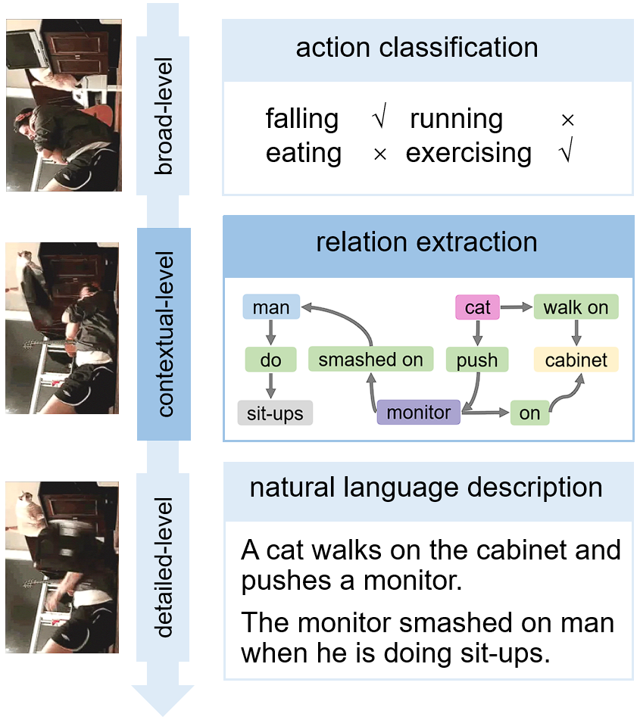
\includegraphics{fig/broad2detail1.png}}
  \caption{Open-vocabulary  Video Relation Extraction enables a contextual-level comprehension of video content, bridging the gap between general action classification and precise language description.}
  \label{fig:motivation}
\end{figure}

\begin{figure}
  \centering
  \resizebox{\linewidth}{!}{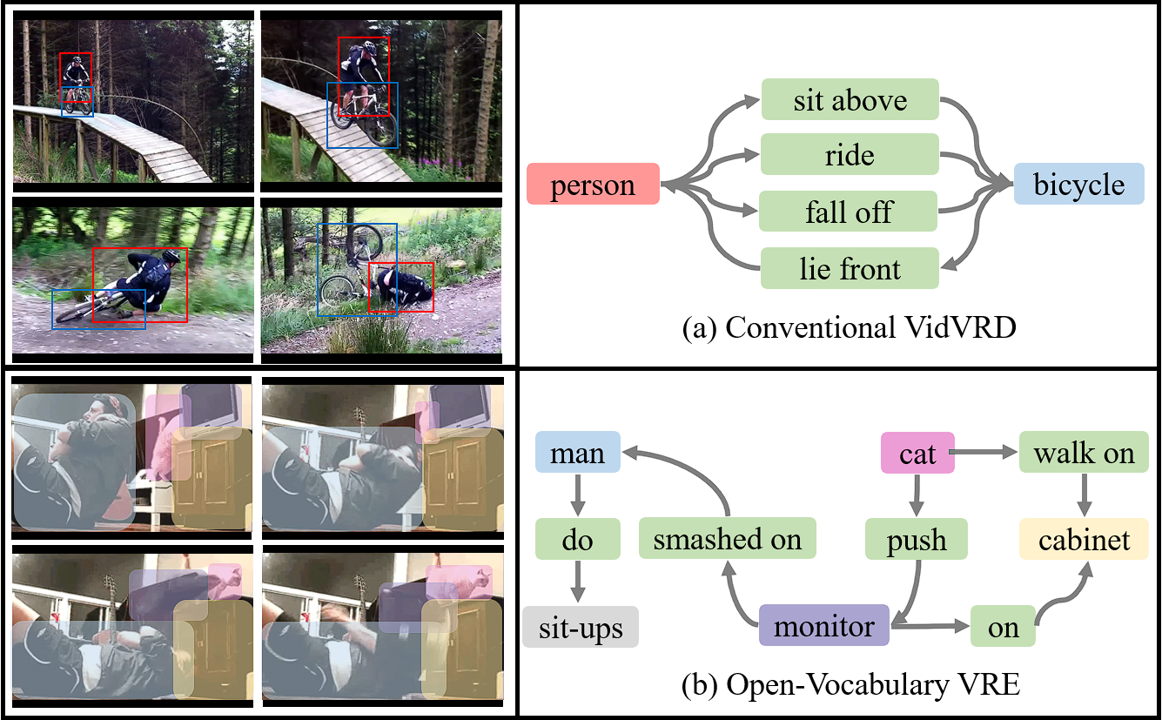
\includegraphics{fig/contra.png}}
  %\caption{Comparisons between VidVRD and OVRE are depicted as follows: (a) A case of VidVRD illustrates object nodes representing the same entity in the relation graph are interconnected throughout frames;
  %(b) An example of OVRE. The relation graph is constructed with a variety of actors and relations that relate to the ``falling'' action.
  \caption{Two \texttt{falling} videos depicted in VidVRD and OVRE diverse in (a) salient objects interconnected throughout frames are exhaustively annotated with diverse relations in VidVRD; (b) OVRE builds a relation graph with various actors and relations that closely related to the falling action.
  %It only needs raw video as input and all nodes in the relation graph are automatically generated.
  }
  \label{fig:compare_anno}
\end{figure}

%任务定义跟解决方案没有关系
%In Natural Language Processing, relation extraction (RE) \cite{DBLP:journals/corr/abs-1712-05191} is a fine-grained task that aims to extract these relation triplets from a piece of unstructured text.
%The traditional pipeline approach considers RE as a two-step problem.
%First, entities are all explicitly presented in the text so they can easily be identified through named entity recognition (NER).
%Second, relation classification (RC) determines whether there exist relationships between entity pairs.
To achieve a comprehensive comprehension of visual content, researchers have introduced Video Visual Relation Detection (VidVRD) tasks~\cite{Shang2017VideoVR,shang2019annotating} specifically designed for video analysis. VidVRD tasks are geared toward identifying objects and the relations between them within videos.
%detect the entities and their relationships presented in a video have been introduced.
%The pipeline of VidVRD is basically the same,
%Nevertheless, as is shown in Figure~\ref{fig:compare_anno} (a), the VidVRD task suffers from the following issues:
% 物体相关,缺乏动作理解
% action genome close-vocab
% problem: 1. object-centric
%VidVRD extensively identifies all relation triplets within the video. For instance, VidVRD~\cite{Shang2017VideoVR} takes available video object detection data and non-exclusively labels all relations between objects, including a bunch of simple relationships. As shown in Figure~\ref{fig:compare_anno} (a), relations such as touch, and watch, are \emph{object-centric} relationships between entities and reveal few implications about the falling action.
%VidVRD extensively identifies all relation triplets within the video.
For instance, VidVRD~\cite{Shang2017VideoVR} employs available video object detection data to non-exclusively label various simplistic relationships between objects. As depicted in Figure~\ref{fig:compare_anno} (a), relationships like \texttt{touch} and \texttt{watch} are inherently \emph{object-centric} relationships with limited implications for the \texttt{falling} action.
Notably, Action Genome~\cite{genome} is distinct in its dedication to an \emph{action-centric} understanding of videos. It dissects actions into spatio-temporal scene graphs. However, it still grapples with a challenge shared by VidVRD – the constraint of a fixed vocabulary range. Consider the scenario shown in Figure~\ref{fig:compare_anno} (a) involving a bicyclist falling from a steep bridge. Due to the vocabulary limitations, the description fails to encompass the bridge and its relationship with the biker, which is an essential element in understanding the falling action.

% From our standpoint, there remains a gap in tasks that enable a contextual-level comprehension of video content coupled with free-form language descriptions.
%The information density differs between language and video \cite{he2022masked}. Languages are human-created symbol systems with rich semantic meaning, whereas videos are natural signals with heavy spatial redundancy, which means objects in videos are implicit information and needed to be manually excavated
% problem: 2. close-vocab
% Action Genome~\cite{genome} is the only one that dedicates to \emph{action-centric} video understanding to our best knowledge. It decomposes the action as a spatio-temporal scene graph. While it still suffers from another problem that hinders VidVRD, that is a fixed range of vocabularies.
%As shown in Figure~\ref{fig:compare_anno} (a), the video depicts two hamsters running on a wheel, and then one of them exits the wheel and starts chewing on food.
%However, due to the limited vocabulary issues mentioned above, terms like ``wheel" and ``chew" will not be included in objects/relations sets of Action Genome.
% For instance, ~\ref{fig:compare_anno} (a) depicts a man who falls off a bike when riding off a steep bridge. However, due to the limited vocabulary problem, it fails to capture the bridge and describes its relation with the biker, which is actually an important factor in falling.
%Most of the existing detectors are only able to detect a limited number of objects. In the meantime, the relationships involved are also predefined as a fixed set. These constraints prevent it from reflecting the complex interactions between objects in the real world accurately.
%Instead, annotators can only choose alternative descriptions such as ``sit next to" or ``walk with", which may not provide effective assistance for VidVRD.

% 介绍新任务的特点
%To alleviate the above limitations of VidVRD, we propose \textbf{O}pen-vocabulary \textbf{V}ideo \textbf{R}elation \textbf{E}xtraction (OVRE), the task of extracting all \emph{action-centric} relation triplets in videos with free-form language descriptions.
%Take Figure~\ref{fig:compare_anno} (b) as an example, OVRE will decompose the video into several relation components: e.g.``\textless \texttt{cat}, \texttt{push}, \texttt{monitor} \textgreater" and ``\textless \texttt{monitor}, \texttt{smashed on}, \texttt{man}\textgreater".
%The only open-vocabulary video understanding task is VidSRL~\cite{vidsitu}, but it focuses on event relations, while OVRE pays more attention to the actions, which is a more fundamental ability for further events understanding.

% To distinguish from previous VidVRD tasks that focus on object-centric relation detection, we borrow the idea from

To mitigate the aforementioned limitations of VidVRD, we introduce \textbf{O}pen-vocabulary \textbf{V}ideo \textbf{R}elation \textbf{E}xtraction (OVRE). OVRE extracts all \emph{action-centric} relation triplets from videos with language descriptions. Take Figure~\ref{fig:compare_anno} (b) as an example: OVRE dissects the \texttt{falling} action into multiple relation components, such as  \textless \texttt{cat}, \texttt{push}, \texttt{monitor} \textgreater and  \textless \texttt{monitor}, \texttt{smashed on}, \texttt{man}\textgreater.
% problem: 3?
%(iii) Annotating bounding boxes in videos is not only expensive but also requires various techniques to simplify \cite{shang2019annotating}. As a result, existing datasets are relatively small in scale.
%In the standard workflow, annotators are typically required to watch the entire video and mark the objects that appear in key frames, connecting them into a series of trajectories.
%Then, given a pair of spatial-temporal annotated objects, annotators need to determine whether there exist relationships between them.
% Introduce our dataset
% 介绍新的数据集的特点
% 1. open-vocab; 2. action-centric
% Since we target at action-centric relation triplets within a video, it is desirable for the video itself to encompass diverse and multiple actions.
% significant inter-class variations in actions, thereby aligning well with our requirements of action understanding.
%In contrast to VidVRD, these are all open-vocabulary annotations.
%In contrast to VidVRD, we have no restrictions on annotations.
%This means that even less frequent words such as ``sit-ups" or ``smash" are possible to be annotated by annotators.
%The key highlight of Moments-OVRE include:
%Through OVRE, video action can now be elucidated using an unrestricted lexicon.
Departing from VidVRD~\cite{Shang2017VideoVR} that confined objects and relations to limited categories, we harness the immense potential of large Language Models (LLMs) to articulate action-aware relations using natural language. In essence, we undertake a two-fold process: first, using CLIP visual encoder to encapsulate video semantics; second, mapping these semantics into the linguistic realm for generating relation triplets through a pre-trained LLM. Employing this straightforward baseline, we achieve the ability to articulate relation triplets with unconstrained vocabularies.

To study OVRE, we present Moments-OVRE, an extensive dataset encompassing over 180K diverse videos.
These videos are sourced from a subset of Multi-Moments in Time~\cite{9609554}(M-MiT), a multi-label video dataset with an average video duration of three seconds.
In Moments-OVRE, we annotate both actors and relations as relation triplets that are most relevant to the action labels without vocabulary limitations. Note that ``actor" does not refer only to human individuals but can also refer to objects, animals, or any entities that are actively involved in an action.
Moments-OVRE confers several advantages:
(\Rmnum{1}) Unrestricted Vocabulary Annotations: Moments-OVRE benefits from an expansive vocabulary encompassing diverse actors and relations, offering a more accurate portrayal of real-world scenarios.
%Moments-OVRE enjoys a large vocabulary of entities and relationships, which can better reflect real-world relations.
(\Rmnum{2}) Emphasis on Action-Centric Annotations: Our annotations exclusively focus on relation triplets related to actions/events depicted in the video.
(\Rmnum{3}) Ample Dataset Scale: Moments-OVRE contains over 180K videos, establishing itself as the most extensive video relation extraction dataset known to date.
% contains 178,480 videos in the training set and 8,463 videos in the test set
% We view OVRE as a one-stage seq2seq process, where the model takes a video as input and generates all the related relation triplets as output.

% Introduce pipelines
% 在数据集的基础上,我们提出了一个模型
%With OVRE, video action can now be elucidated using an unrestricted lexicon. It involves the open-vocab description of videos, past VidVRD methods~\cite{Shang2017VideoVR} that classify objects and relations within limited categories are no longer feasible. Thus we harness the remarkable capabilities of large LLMs to describe action-aware relations with natural language. Simply put, we pre-train the visual encoder of a CLIP model for representing video semantics, which is further mapping to the language domain for relation triplets generation with a pre-trained LLM. With this simple baseline, we are able to describe action-centric relation triplets with free-form vocabularies.


% Summary
The main contributions are as follows:

\textbullet \ We introduce the novel Open-vocabulary Video Relation Extraction task, aiming to extract action-centric relations within videos. %Moreover, we introduce a range of evaluation metrics to facilitate robust assessment.
%to-date largest

\textbullet \ To foster ongoing research, we curate Moments-OVRE, an expansive dataset for video action comprehension. Comprising over 180k videos, Moments-OVRE is enriched with comprehensive open-vocabulary relationship annotations.
%We create a large video action understanding dataset, Moments-OVRE, to facilitate further research. Moments-OVRE consists of 180K diverse videos, along with extensive open-vocabulary relationship annotations.

\textbullet \ We build a simple pipeline designed for generating action-centric relation triplets from raw videos. Extensive experimentation is conducted to validate assorted design considerations employed within the pipeline.


%相关工作可以写满半栏+,目前不够
\section{Related Works}
%We organize our related as ""

% \textbf{On the Task: Video Understanding}
% list different tasks and analyse the correspondence/difference between them.
% Hightlight our task is first proposed.

% \textbf{On the Method: Relation Extraction}
% img/video relation extraction methods{list}
% type:
% 1. Scene Graph
% 2. Seq2Seq/generation
% ours:

% \textbf{On the Dataset: Understanding Benchmarks}
% Tab.1
% introduce the different benchmarks and highlight the difference of our benchmark especially "open-vocabulary".



%Introduction
%p1, p2: background ---> our motivation
%  ----------video understanding Task Overview-------
% --------------------------------------------------->
% task: action       relation     caption
% example: video + label
% level: coarse(*) [mid-level(**)](highlight)  fine-grained(***)

% p3,p4: ours task & benchmark

% p5: method

% p6: contribution


% Else:
% paper name: OVRE
% Moments-OVRE --> Moments-OVRE (dataset name)


%Video understanding has always been an active research area in the field of computer vision, involving various tasks with different levels of granularity.
% 这里不应该描述数据集的构建时间,而应该介绍数据集的动作类别特点
\begin{table*}[t]
    \centering
    \caption{Representative video understanding datasets.}
    \begin{adjustbox}{width=\textwidth}
    \begin{tabular}{cccccccc}
        \toprule
        Dataset & Task & Annotation & \#Video & \#Subject/Object & \#Predicate & Avg. Time (s) & Source \\
        \midrule
        Kinetics400 & \multirow{2}{*}{Action Classification} & \multirow{2}{*}{Action Categories} & 306,245 & - & - & 10 & YouTube\\
        %Sth-Sth V2 &  &  & 220,847 & - & - & 4 & Crowd-workers\\
        VideoLT &  &  & 256,218 & - & - & 192 & YouTube\\
        \midrule
         MSR-VTT & \multirow{2}{*}{Video Captioning / Retrieval} & \multirow{2}{*}{Textual Descriptions} & 7,180 & - & - & 20 & Web\\
         %M-VAD &  &  & 48,986 & - & - & 6 & DVS\\
         VATEX & & & 41,269 & - & - & 10 & YouTube\\
        \midrule
        VidVRD & \multirow{3}{*}{Video Visual Relation Detection} & \multirow{3}{*}{BBoxes, Relation Triplets} & 1,000 & 35 & 132 & 33 & ILVSRC2016-VID\\
        VidOR & & & 10,000 & 80 & 50 & 35 & YFCC100M\\
        Action Genome & & & 10,000 & 35 & 25 & 30 & Charades\\
        \midrule
        VidSitu & Video Semantic Role Labeling & Verbs, SRLs, Event Relations & 29,220 & Open & Open & 10 & Condensed-Movies\\
        \midrule
        \textbf{Moments-OVRE} & \textbf{Open-Vocabulary Video Relation Extraction} & \textbf{Relation Triplets} & \textbf{186,943} & \textbf{Open} & \textbf{Open} & \textbf{3} & \textbf{M-MiT}\\

        \bottomrule
        \\
    \end{tabular}
    \end{adjustbox}
    %removedVspace
    \label{tab:dataset_comp}
\end{table*}

\textbf{Video understanding} has long been an active research area in computer vision, encompassing a wide range of diverse aspects.
Action recognition~\cite{Kay2017TheKH,8237884,monfortmoments} categorizes the video content into a predefined set of action classes, temporal action localization~\cite{Hei2015anet,liu2022fineaction} further emphasizes the specific time points at which these actions occur.
Tasks such as video captioning~\cite{chen2019deep}, video question answering~\cite{qian2023locate}, and video-text retrieval~\cite{song2021spatial} are dedicated to learning a detailed representation of semantic information.
%focus on overall video comprehension and are particularly concerned with representing semantic information at a more detailed level.
%Between these tasks lies an intermediary area known as relation understanding, which aims to capture the diverse relationships between objects.
In the spectrum of these tasks resides an intermediary domain referred to as relation understanding,  dedicated to capturing the diverse relations among objects.
This contextual domain provides semantically rich intermediate representations for videos, crucial for comprehending interactions and behaviors depicted within them.
VidVRD~\cite{Shang2017VideoVR} and VidOR~\cite{shang2019annotating} are representative benchmarks for relation understanding, with finite object and predicate sets.
Recently proposed task Open-VidVRD \cite{gao2023compositional} manually splits the finite object and predicate sets into base and novel categories and builds the novel prediction setting.
However, these existing VRD tasks focus on object-centric relation detection and struggle to bridge the gap between closed-label sets and natural languages, prompting us to propose video relationship extraction under open-vocabulary scenarios.
%In general, unlike Video Captioning, which focuses on the overall video comprehension, and VidVRD, which focuses on object-centric relation detection under fixed subjects/objects and predicates sets, \textbf{OVRE} mainly aims at identifying informative triplets in videos that characterize various actions.
Moreover, we aim to identify informative triplets that portray various actions in the video.

\noindent \textbf{Contextual-level Visual Comprehension} has been mainly explored in the image domain, including scene graph generation~\cite{genome}, visual semantic role labeling~\cite{yatskar2016situation, sadhu2021visual}, and human-object interaction~\cite{li2022hake, gkioxari2018detecting}. These tasks have also been extended to the video domain, which requires information aggregation across frames.
Existing works often treat video relation detection as a multi-stage pipeline, including object tracking, tracklet pair generation, and relation classification. These works focus on improving relation classification by leveraging contextual knowledge~\cite{10.1145/3343031.3351058} or adding additional modules to enhance predicate representation~\cite{gao2021video} with generated tracklets.
%while simply employ a pretrained Faster-RCNN~\cite{ren2015faster} and deepSORT~\cite{wojke2017simple} algorithm to generate a series of tracklets.
Recent trends lean towards one-stage models like VRDFormer~\cite{zheng2022vrdformer}, employing various queries to integrate spatio-temporal information, facilitating tracklet pair generation and relation classification concurrently.
%Nevertheless, these methods are constrained by the limited number of objects and relationships present in the datasets, which hinders their scalability and generalization.
However, their scalability and generalization are hampered by datasets containing a restricted size of objects and relationships.
Video captioning, aimed at generating open-ended descriptions, typically uses an encoder-decoder architecture. Over time, this setup has advanced to more sophisticated models~\cite{zhang2019reconstruct,tang2021clip4caption,lin2022swinbert}. %focuses on generating open-ended language descriptions and existing methods often utilize an encoder-decoder architecture to generate fluent language expression. Over the years, video encoder and text decoder have been continuously replaced by more advanced models \cite{zhang2019reconstruct,tang2021clip4caption,lin2022swinbert}.
Recent strides in visual-language representation learning have led to models pre-trained on extensive paired data demonstrating promise in fine-tuning for various multi-modal tasks~\cite{wang2022git,xu2023mplug2,chen2023valor}.
%With the significant progress in visual-language representation learning, models pre-trained on massive paired visual-language data have achieved promising results when fine-tuning different multi-modal downstream tasks~\cite{wang2022git,xu2023mplug2,chen2023valor}.
Building on the progress in video captioning, we seek to leverage generative models for our OVRE task.

\noindent \textbf{Datasets for video understanding} have been introduced in support of multiple tasks over the past years.
Kinetics400 \cite{Kay2017TheKH} is a widely adopted category-balanced classification dataset. VideoLT~\cite{zhang2021videolt}, in opposition, follows a naturally long-tailed distribution for action recognition.
%M-VAD~\cite{yue2023movie101} comprises video clips from 92 movies and aligns them with descriptions via a semi-automatic procedure DVS.
MSR-VTT \cite{7780940} is a widely adopted dataset for video captioning and video retrieval, it includes video clips from different domains, and each of them is annotated with approximately 20 natural sentences. Recently introduced VATEX~\cite{wang2019vatex} is a large-scale multilingual video description dataset.
VidVRD \cite{Shang2017VideoVR} and VidOR~\cite{shang2019annotating} densely annotate objects and the most basic relations.
Action Genome~\cite{genome} focuses on action understanding by decomposing them into different relationships and ignoring others that are irrelevant to actions.
VidVRD datasets have restricted their objects and relations to a fixed label set and thus are far away from reflecting the diverse relations in the real world.
VidSRL~\cite{sadhu2021visual} presents the sole open-vocabulary relation understanding task, while it primarily focuses on events. In contrast, OVRE places greater emphasis on actions, which is a fundamental ability for event comprehension.
Detailed statistics for these datasets are listed in Table~\ref{tab:dataset_comp}.

% % FCVID也有动物景观之类的标签,involve的意思不够明确,MiT应该没有这些标签
% Moments in Time \cite{monfortmoments} contains 1M short video clips with 339 action categories.
% Multi Moments in Time (M-MiT)\cite{9609554} was released as a multi-label extension of Moments in Time afterward. It removes actions with semantic ambiguity and merges similar actions, resulting in 292 distinct action classes.
% Unlike other datasets designed only for human action,  they encompass a significant intra-class variation among the categories and thus understanding actions in these videos is more challenging.
% For instance, the subject of swimming could be a person, a fish, or an animated character.

%
%
% MSR-VTT \cite{7780940} includes video clips from different domains, and each of them is annotated with approximately 20 natural sentences.
% There have also been datasets that focus on more fine-grained dense captioning. For example, ActivityNet Captions \cite{DBLP:journals/corr/KrishnaHRLN17} have 20K untrimmed videos. Each video has at least 3  temporal localized captions.

% \textbf{Video Visual Relation Detection} (VidVRD) aims at understanding entities and relationships within videos by parsing them into scene graphs.
% VidVRD \cite{Shang2017VideoVR} is the first dataset introduced for this task with densely annotated object bounding boxes and relation triplets. It focuses on the most basic relations and expands them in spatial dimensions. For instance, the relation ``run" has variants like ``run left'', ``run front'' etc.

% VidOR \cite{shang2019annotating}  improves the annotation strategy and thus significantly expands the scale and relation categories of the dataset.

% Unlike the aforementioned datasets, Action Genome~\cite{genome} focuses on action understanding by decomposing them into attention, spatial, and contact relationships.
% % Action Genome is built upon Charades, which means it cares more about human relations and ignores other relationships that may be important for understanding diverse actions.
% However, all of these datasets have restricted their objects and relations to a fixed label set and thus are far away from reflecting the diverse relations in the real world.
% Although VidSRL~\cite{vidsitu} represents the sole open-vocabulary video comprehension task, it primarily focuses on event relations. In contrast, OVRE places greater emphasis on actions, which serves as a fundamental skill for comprehending subsequent events.
% In Table~\ref{tab:dataset_comp}, we provide detailed statistics on related datasets.


\section{Video Relation Extraction Benchmark}
 %In this section, we brief the definition and evaluation metrics of the OVRE task.
\subsubsection{Task Formulation}
Given a raw video input $V$, OVRE targets inferring its corresponding visual relationships $R$. Here, $V\in\mathbb{R}^{T\times H\times W\times C}$ denotes its frame sequence, where $T$, $H$, $W$, and $C$ represent the number of frames, width, height, and channels respectively. The relation triplets are represented as $R=\{{r_{1}},\cdots,{r_{K}}\}$, and each relation $r_{K}$ is structured as a triplet:  \textless \texttt{subject}, \texttt{relation}, \texttt{object}\textgreater.
%$R=\{r_{k}\}_{k=1}^{K}$ is a collection of relation triplets and each relationship is formed as a triplet ``\textless \texttt{Subject}, \texttt{Relation}, \texttt{Object}\textgreater''.
%Our target is to learn the generation of $R$ for the input video.

%In contrast to caption descriptions, videos can encapsulate numerous relationships. Each relation consists of a sequence of words $w=\{w_{1},w_{2},...,w_{N}\}$. These relations are then concatenated to form a token sequence $R=w_{1},w_{2},...,w_{M}$, with tokens being padded to a maximum length of $M$.

%Cause actions within videos can convey diverse interactions and different interactions can be shared by different actions, we intend to extract all the relations that are related to actions within videos.
Given that actions depicted in videos can encompass a wide spectrum of interactions, and distinct interactions might be common across various actions, our objective is to systematically extract all relationships associated with actions within the video context.
Each $r_{i}$ consists of a sequence of words $w=\{w_{1},w_{2},...,w_{N}\}$. These individual $r_{i}$ are then concatenated to form a token sequence $R=w_{1},w_{2},...,w_{M}$, which serves as a representation of a sequence of relation triplets, collectively portraying all the action-centric relationships.
%to represent a relation triplet sequence depicting all the action-centric relations.
The training objective is to maximize the likelihood of generating $R$ given the video $V$:
$$
\underset{\theta}{\max} \log p_{\theta}(R|V),
$$
where $\theta$ denotes the model's trainable parameters.
Our key idea is to leverage the powerful capability of generative models to address the OVRE problem.
Consequently, the revised training objective can be formulated as follows:
%Thus, the training objective can be rewritten as:
$$
\underset{\theta}{\max}\sum_{i=1}^{M}\log p_{\theta}(w_{i}|V,w_{i-1}).
$$
OVRE involves generating relationships using nature language, rendering common metrics wildly used VidVRD metrics such as Precision@K and Recall@K unsuitable for our task.
Inspired by the evaluation metrics in image captioning, we advocate for assessing the quality of generated triplets using Bleu, CIDEr, and METEOR scores.
For the Bleu metric, we only consider B@1, B@2, and B@3, as each triplet contains at least three words.
These metrics face challenges when applied directly to evaluating the overall relation triplets since the generated triplet sequence can be regarded as an unordered set, whose alignment with the ground truth triplets is unknown.
% cannot be directly applied to evaluate the generated relation triplets

\begin{figure}[t]
  \centering
  \resizebox{1.0\linewidth}{4cm}
  {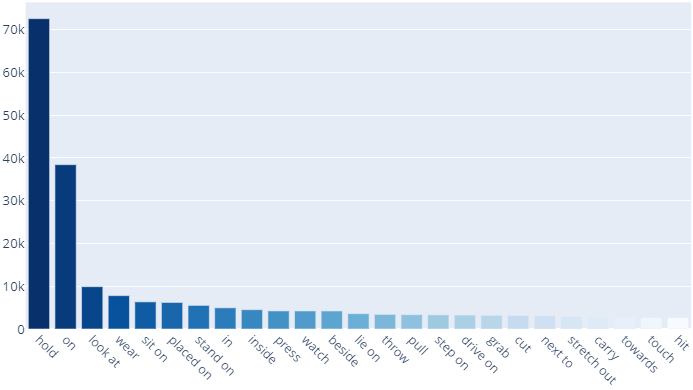
\includegraphics{fig/rel.png}}
  \caption{Counts of top 25 relationships in Moments-OVRE.}
  \label{fig:freq}
\end{figure}

To match the generated triplet set with the ground truth,
%since we have concatenated all the relation triplets together into a whole sequence, and the relation triplets themselves are unordered.
%To build a better evaluation pipeline, it is necessary to separate each triplet from the generated sequence and match them with ground truth ones.
% 缺少对这种做法的合理性的讨论
we first utilize a sentence embedding model SimCSE \cite{gao2021simcse} to quantify the text similarity between the generated and ground truth triplet set.
Then we use these embeddings to acquire a similarity matrix $S$, where $S_{ij}$ denotes the cosine similarity score of generated triplet $\hat r_i$ and ground truth triplet $r_{j}$.
After obtaining $S$, we use the Hungarian algorithm to establish one-to-one matches between the triplets and apply the aforementioned metrics to these paired triplets.
%This similarity matrix subsequently forms the foundation for employing the Hungarian algorithm, enabling the establishment of one-to-one matches between the triplets. Consequently, the aforementioned metrics can be applied to this aligned set of paired triplets.
%Note that the number of generated triplets may not always equal that of ground truth. When there are more ground truth triplets, we simply assign a score of 0 to the remaining unmatched ones.
Note that the number of generated triplets may differ from that of ground truth triplets. When fewer triplets are generated, unmatched ground truth triplets receive zero scores.

\section{Dataset Construction}
We present the Moments-OVRE dataset tailored for OVRE. Notably, Moments-OVRE boasts distinct attributes such as diverse video content, an extensive compilation of video-triplet pairs, annotations embracing open vocabulary, and a focus on action-centric relationships.
%Moments-OVRE is characterized by unique properties including varied video content, large-scale video-triplet pairs, open-vocabulary and action-centric annotations.
In this section, we will detail how we select representative videos, annotate relations, and devise data splits. Additionally, we thoroughly explore and analyze the statistical insights within the Moments-OVRE dataset.
%We also present and analyze various statistical data in Moments-OVRE.

\subsubsection{Video Selection}
Since our task focuses on action-centric relationships, several requirements are posed for the selection of videos.
First, we prefer videos with multiple actions. Second, videos should contain rich information, involving different scenes, objects, and events in the real world.
%First, videos shouldn't depict the same action throughout the entire time sequence, as it would significantly reduce the diversity of relationships.
%Second, videos should by themselves contain rich information, involving different scenes, objects, and events in the real world.
%Considering all these factors, we exclude domain-specific datasets such as YouCook and Howto100M \cite{DBLP:journals/corr/abs-1906-03327} and single-label datasets such as Kinetics and Something-Something.
% are also excluded since most of their videos only concern a single action.
We choose to annotate videos from Multi Moments in Time (M-MiT) \cite{9609554} due to its multi-label nature, which allows a more nuanced comprehension of actions within intricate contexts.
%action understanding under more complex scenarios.
M-MiT offers several distinct advantages:
%(i) M-MiT encompasses a significant intra-class variation compared to other commonly used datasets such as Kinetics, which means a detailed description of relationships will force the model to explore such variation among videos with the same action labels.
%(ii) The majority of videos in M-MiT have a duration of only 3s, making the annotators concentrate more on depicting the action rather than the temporal context, which is more common for long-duration videos of YouCook and Howto100M.
(\Rmnum{1}) Unlike commonly utilized action datasets like Kinetics, M-MiT exhibits substantial intra-class diversity. This highlights the necessity of providing more intricate descriptions of relationships to capture variations between videos of the same action labels.
(\Rmnum{2}) A majority of M-MiT videos have a duration of only 3 seconds. This temporal brevity encourages annotators to focus primarily on portraying the action itself, as opposed to the temporal context which is more prevalent in longer videos, such as those in YouCook and Howto100M datasets.
%in them highly convenient for viewing and annotation.
%Additionally, the brevity of videos minimizes the impact of contextual factors on the annotation process.
% Short videos make the annotation less influenced by the context surrounding the video.
Considering the long-tail distribution of action categories in M-MiT, we attempt to relatively balanced sampling videos from all classes. M-MiT has 292 action categories, we sample at least 660 videos per class and additionally select other random videos as some videos may be discarded during annotation.
%As a certain number of categories had fewer samples than the average, we supplement them by sampling from other categories.
\begin{figure}[t]
  \centering
  \resizebox{0.85\linewidth}{!}{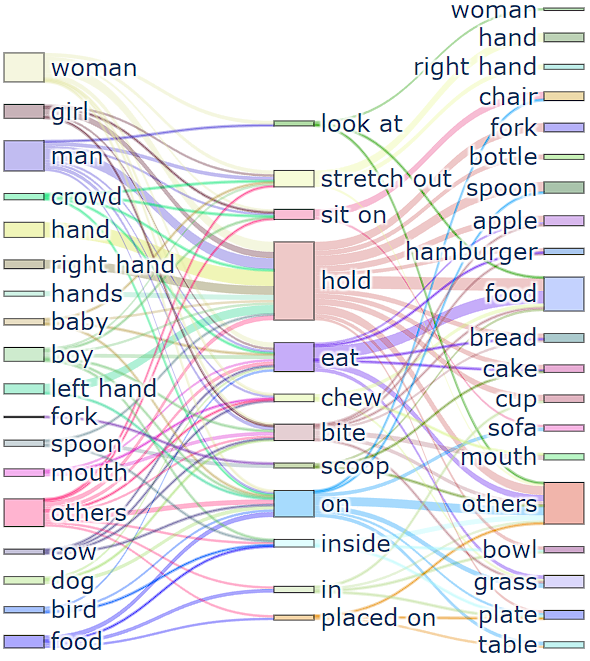
\includegraphics{fig/eating.png}}
  \caption{A weighted bipartite mapping of the top 12 most frequent relations in \texttt{eating} videos.}
  %\caption{A weighted bipartite mapping between objects and relationships shows that they are densely interconnected in Action Genome. The weights represent percentage of occurrences in which a specific object occurs in a relationship.}
   \label{fig:sanki}
\end{figure}
\subsubsection{Annotation Pipeline}
% We perform action-centric annotation.
%We randomly shuffled all the categories and assigned a batch of 200 videos to each annotator for annotation.
We ask annotators to perform an action-centric relation triplet annotation, which follows these steps:
Given the potentially noisy nature of the large-scale M-MiT dataset, annotators first verify the correctness of the action labels. Videos with incorrect labeling are subsequently excluded.
To perform action-centric annotation, both the video and the corresponding action labels are presented to the annotators. They first identify and annotate all pertinent objects, and then articulate the associated relationships among these objects.
Annotators are instructed to provide descriptions for relation triplets solely when these relationships are relevant to the action labels.
To illustrate, refer to Figure~\ref{tab:dataset_comp} (b): the annotation \textless \texttt{monitor}, \texttt{smashed on}, \texttt{man} \textgreater is required, whereas the annotation \textless \texttt{guitar}, \texttt{placed on}, \texttt{ground} \textgreater is invalid, as the latter constitutes background information rather than being directly tied to the \texttt{falling} action.
% Through this methodology, we ultimately acquire visual relation triplets that are closely related to the action labels. Refer to the Appendix for more comprehensive details.
Besides, we also manually review and correct the low-quality annotations.
% Our annotation pipeline is as follows:
% While not all videos in M-MiT are correctly labeled, the annotators should first check the correctness of action labels. Mislabeled videos are considered invalid data and will be filtered from our dataset.
% We present both the video and the accompanying action labels to the annotators.
% They should first annotate all the relevant objects to form a list of objects, then describe all related relations among these objects.
% Annotators are reminded to describe the relation triplets if and only if these relationships are related to the action labels.
% Take Figure~\ref{tab:dataset_comp} (b) as an example, annotations such as ``monitor smashed on man" are allowed while ``guitar placed on ground" is not, as it is actually background information of the video action.
% In such a way, we can finally obtain the visual relation triplets that are tightly relevant to the action labels. See Appendix 1 for details.
% It should be noted that some relationships reflected by specific action categories cannot be expressed as subject, predicate, or object.
% We allow such annotations, and padding a special token XXX for the predicate.

\subsubsection{Dataset splits}
The data is partitioned into training and testing sets, resulting in 178,480 and 8,463 videos respectively.
To ensure maximum consistency with the original splitting, all videos are selected exclusively from their designated sets within the M-MiT collection.
%all these videos are sourced from their respective sets within M-MiT.
\begin{figure*}[t]
  \centering
  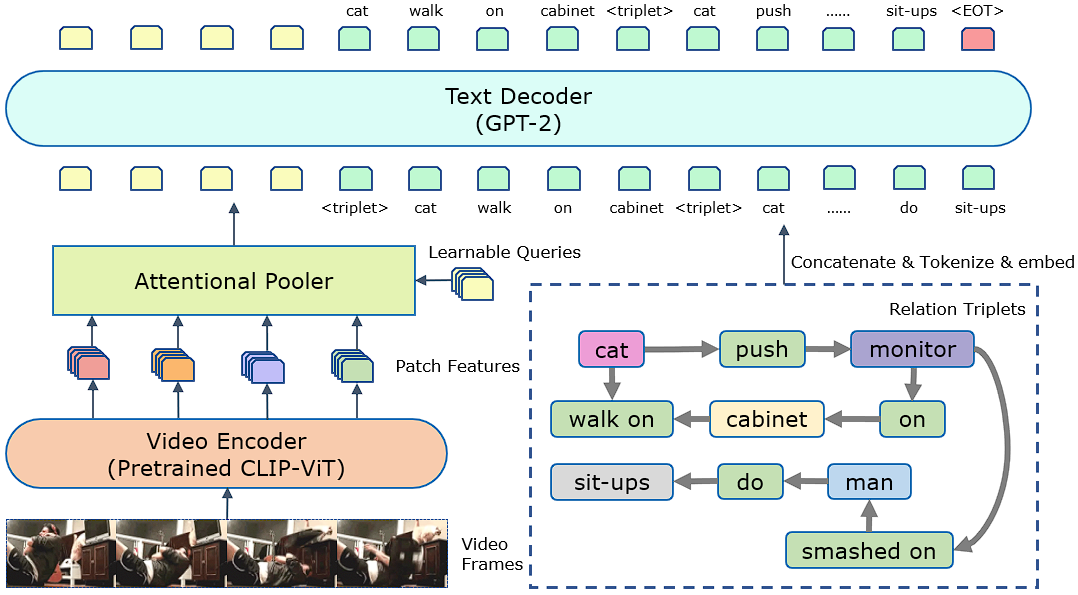
\includegraphics[width=0.9\textwidth]{fig/model-.png}
  \caption{Overview of our model architecture, enabling simple relation generation with the powerful vision-language pre-trained model CLIP-ViT as the video encoder and the large language model GPT-2 as the text decoder.
  %We train a query-based transformer to extract fine-grained information from CLIP patch features. Given the queries and word tokens, we perform self-attention through the text decoder and predict the word tokens.
  }
  \label{fig:arch}
\end{figure*}

\subsection{Dataset Analysis and Statistics}
Overall, Moments-OVRE offers open-vocabulary annotations for 186,943 videos, encompassing a sum of 399,576 relation triplets.
In Figure~\ref{fig:freq}, we show the distribution of the top 25 most frequent relations in Moments-OVRE, which follows a natural long-tailed distribution. Furthermore, Figure~\ref{fig:sanki} shows frequently described relation triplets of \texttt{eating} videos. Note that \texttt{hold} is a prevalent visual relation shared by various kinds of videos, such as \texttt{painting}, and \texttt{drinking} videos. A clue from this observation is that merely relying on a single relation is insufficient to infer the action categories from the videos, and a comprehensive understanding requires recognition of combinations of diverse relations.
%\texttt{hold} relation but also other contextual relations like \texttt{chew} and \texttt{bite}.

%``holding'' action is not enough while cooperating with the action context is crucial for a genuine understanding of the video actions.
%In Figure~\ref{fig:freq}, we visualize the distribution of the top 25 most frequently occurring objects and relations within the dataset. As is common with many datasets, objects and relations exhibit a long-tailed distribution. Furthermore, we compare relations triplets in Moments-OVRE and those in Visual Genome~\cite{genome}. This contrast is illustrated in Figure~\ref{fig:compvg}, revealing that VG has more annotations on the spatial relations while Moments-OVRE pays more attention to action understanding.
%We present an extensive analysis of Moments-OVRE. Overall, we provide open-vocabulary annotations of 186,943 videos, yielding a total of 399,576 relation instances. In Figure~\ref{fig:obj+rel}, we visualize the distribution of the most frequently occurring 25 objects and relationships in the dataset. Similar to most datasets, some objects, and relationships appear more frequently than others.
%We also compare the relationships of our Moments-OVRE with those in Visual Genome (VG). As can be seen from Figure~\ref{fig:compvg}, VG has more annotations on the spatial relations while Moments-OVRE pays more attention to action understanding.
% word frequency
% object classes(non-unique descriptions, frequency>5?)?
% relation classes?
% some videos are annotated in a very detailed way?
\section{Method}
\subsubsection{Overview}
An illustration of our method is provided in Figure~\ref{fig:arch}. The overall framework mainly includes a Video Encoder, an Attentional Pooler, and a Text Decoder.
The video is first transformed into a sequence of features via the video encoder.
These features are further condensed into prefix information by the attentional pooler, which is then fed into the text decoder for relation triplet generation.
% \emph{Following recent research \cite{DBLP:journals/corr/abs-2111-09734}, we also encode the video as prefix information and utilize a language model to sequentially predict the subsequent tokens.}

\subsubsection{Video Encoder}
%CLIP \cite{DBLP:journals/corr/abs-2103-00020} has been pre-trained via an unsupervised contrastive loss over 400M image-text pairs from the web.
To extract visual features from a video, we leverage the visual encoder of a pre-trained CLIP \cite{radford2021learning} model.
Previous research has demonstrated its exceptional performance across various open-vocabulary recognition tasks \cite{ni2022expanding,tang2021clip4caption,luo2022clip4clip}.
% We choose CLIP-ViT to extract visual information from a video. ViT\cite{DBLP:journals/corr/abs-2010-11929} transmit video frame into a sequence of patches. Visual patches contain more fine-grained information and thus are a better choice for OVRE. Then, with the additional temporal dimension, a video $V\in \mathbb{R}^{T\times H\times W}$ will results in $(T\times\frac{HW}{P^{2}}=786)$ patches.
Our choice for visual feature extraction is CLIP-ViT, which utilizes ViT\cite{dosovitskiy2020image} to translate video frames into sequences of patches. These visual patches capture finer-grained information, making them an optimal fit for OVRE. However, the incorporation of the temporal dimension necessitates consideration of the resultant number of patches. Specifically, for a video $V\in \mathbb{R}^{T\times H\times W}$, this translates to $T\times\frac{HW}{P^{2}}$ patches.
\subsubsection{Prefix Strategies}
With the features from $V$, our focus shifts towards transmitting them into the textual domain for relation generation. A simple solution is to directly feed all patches into the decoder, while the excessive number of patches not only leads to additional computational costs but also introduces a lot of redundant information.
In light of this, we utilize an attentional pooler denoted as $F(\cdot)$, which employs a predetermined number of queries to extract meaningful features from all video patches:
$
q_1,...,q_m=F(p_1,...,p_n,q_1,...,q_m),
$
which aggregates spatial-temporal features into a more concise representation.
\subsubsection{Attentional Pooler}
Drawing inspiration from the approach introduced in VideoCoCa \cite{yan2023videococa},
our framework incorporates an essential element known as the Attentional Pooler. This module takes learnable queries and patch features as its input, facilitating cross-attention mechanisms between them.
The optimization of both the parameters of the Attentional Pooler and the queries enables the queries to gradually refine their ability to extract significant relationships from the patches. This design proves well-suited to the demands of OVRE. Remarkably, even with a single-layer transformer, our model showcases its ability to generate a diverse set of meaningful visual relationships.
% One of our key components is the Attentional Pooler adopted from VideoCoCa \cite{yan2023videococa}, which is essentially a lightweight transformer.
% It takes learnable queries and patch features as input and performs cross-attention among them.
% By simultaneously optimizing the parameter of the Attentional Pooler and queries, the queries can eventually learn to retrieve meaningful information from patches.
% We found that this design is suitable for OVRE and even when using a single-layer transformer, our model is able to generate diverse and meaningful visual relationships.



\subsubsection{Text Decoder}
We employ GPT-2 \cite{radford2019language} as our generation model.
Though relationships themselves are unordered, we observe that sorting them by Triplet Linearization \cite{cabot2021rebel} does not provide significant benefits in OVRE.
Accordingly, all relation triplets of a video are simply concatenated into a text sequence by a separation token.
Then, we map all the words into their corresponding tokens and pad them to the maximum length $M$ to obtain a sequence of embeddings.

\section{Experiments}
%In this section, we present the evaluation results of our methods and baseline models on our Moments-OVRE. We also report the result of the ablation studies of our methods.
\subsection{Experiments Settings}
\noindent\textbf{Video and Text Preprocessing. }
For each input video, we first resize it to 224 $\times$ 224 and then extract 16 frames using uniform sampling, resulting in 786 patches for each video. We utilize RandAugment \cite{Ekin2019randaugment} as our data augmentation strategy.
For the paired relation triplets, we concatenate the unordered relation triplets into a sequence using the special token \textless\texttt{triplet}\textgreater.

\noindent\textbf{Training Setting. }
We train the generation model using cross-entropy loss and employ teacher forcing to accelerate the training process.
All models are optimized using AdamW optimizer, with $\beta_{1}=0.9$, $\beta_{2}=0.999$, a batch size of 16, and weight decay of 1e-3.
The initial learning rate is set to 1e-6 for CLIP, 2e-5 for GPT-2, and 1e-3 for AttentionPooler.
We applied learning rate warm-up during the early 5\% training steps followed by cosine decay.
We trained the networks for 50 epochs on 8 Nvidia V100 GPUs and chose the model with the highest CIDEr score as the final model.

\begin{table}[t]
    \centering

    \begin{tabular}{cccccc}
        \toprule
        Method & B@1 & B@2 & B@3 & CIDEr & METEOR \\
        \midrule
        ClipCap & 29.75 & 16.32 & 9.48 & 125.45 &  19.25\\
        GIT & 35.19 & 20.12 & 11.90 & 155.38 & 23.06 \\
        \textbf{Ours} & \textbf{37.27} & \textbf{21.92} & \textbf{13.90} & \textbf{174.47} & \textbf{25.07} \\
        \bottomrule
        \\
    \end{tabular}
    \caption{Baseline comparison on Moments-OVRE.}
    \label{tab:main_res}
\end{table}
\begin{table}[t]
    \centering

    \begin{tabular}{cccccc}
        \toprule
        CLIP & GPT2 & CIDEr & METEOR \\
        \midrule
         \ding{55} & \ding{55} & 131.85 &  19.84\\
        \ding{55} & \ding{51} & 165.67 & 24.12 \\
       \ding{51} & \ding{51} & \textbf{174.47} & \textbf{25.07} \\
        \bottomrule
        \\
    \end{tabular}
    \caption{Study on vision and language model fine-tuning. The \ding{51} mark means fine-tuning the corresponding module.}
    \label{tab:abl_ft}
\end{table}
\begin{table}[t]
    \centering

    \begin{tabular}{ccc}
        \toprule
        Features & CIDEr & METEOR \\
        \midrule
        Region & 77.38 & 13.14 \\
        Frame & 115.85 &  18.11\\
        Patch & \textbf{165.67} & \textbf{24.12} \\
        \bottomrule
        \\
    \end{tabular}
    \caption{Comparisons with different visual features (w/o fine-tuning visual encoder).}
    \label{tab:abl_feat}
\end{table}

\subsection{Main Results}
\noindent\textbf{Baselines models. }
Previous VidVRD methods focused on predicting relationships over detected objects, which is essentially a classification task and thus cannot be applied to OVRE.
Therefore, we introduce several generative models as baseline models.

\textbullet  \ ClipCap \cite{mokady2021clipcap} is an image captioning model that utilizes the same visual encoder and text decoder as we do.
It uses a mapping network to convert CLIP embeddings into GPT-2 prefixes.
To apply ClipCap for videos, we follow the most common strategy that treats each video frame as an individual image and then perform a mean pooling layer along the temporal dimension to obtain a global video representation.

\textbullet  \ GIT \cite{wang2022git} stands as a vision-language generative model, demonstrating strong performance across numerous generation tasks. This achievement is attributed to its effective optimization of the language model loss during pre-training, involving a substantial collection of image-text pairs.
%GIT \cite{wang2022git} is a vision-language generative model.It performs well in many generation tasks by optimizing the language model loss under massive image-text pairs in the pre-training stage.
We directly fine-tune $\text{GIT}_{\text{B}}$ to generate relation triplets without making further modifications.

% \textbullet \textcolor{blue} {VALOR \cite{chen2023valor} is a unified vision-audio-language pretraining model which unifies tri-modality undersatanding and generation through Multimodal Grouping Alignment and Multimodal Grouping Captioning. Since more than half of the videos in the moments dataset have no audio information, for this case, we use blank audio to replace the audio input of VALOR model.}
% However, this approach is suboptimal since it only focuses on the overall information of the video, while
% OVRE requires the model to pay more attention to the objects and their interactions.

% ---
% Baselines & Freeze
%            & FT
% Competitor (Video Cap) & M1
%                        & M2

% Competitor (To Do)  & M1
%                        & M2

% Ours &
% ---

\noindent\textbf{Result and Analysis. }
We present our results on Moments-OVRE in Table~\ref{tab:main_res} and compare our approach with baseline methods trained under the same training settings.
Our approach outperforms baseline generative methods, achieving a higher METEOR score (+6.22) than ClipCap and (+2.01) than GIT.
We find that although GIT was pre-trained on 0.8B image-text pairs and achieved impressive performance on video captioning datasets, it did not perform as well as our approach on the OVRE task. This could be attributed to the fact that the image-text generative pre-training does not directly facilitate the understanding of fine-grained information such as relationships in videos.
% we highlight several points.
% 1) We are best. Compared with baselines and xxx, we perform .. Achieve xx\% on data.
% 2) Ft is better than Freeze. (analyse) + so why also finetune the backbone in our method
% 3) As the performance of video caption based methods, we find xxx. They also perform xx, they can also generate some reasonable. But, worse than us. Analyse, 1) long caption, ours: triplet.

\begin{figure}
  \centering
  \resizebox{0.85\linewidth}{!}{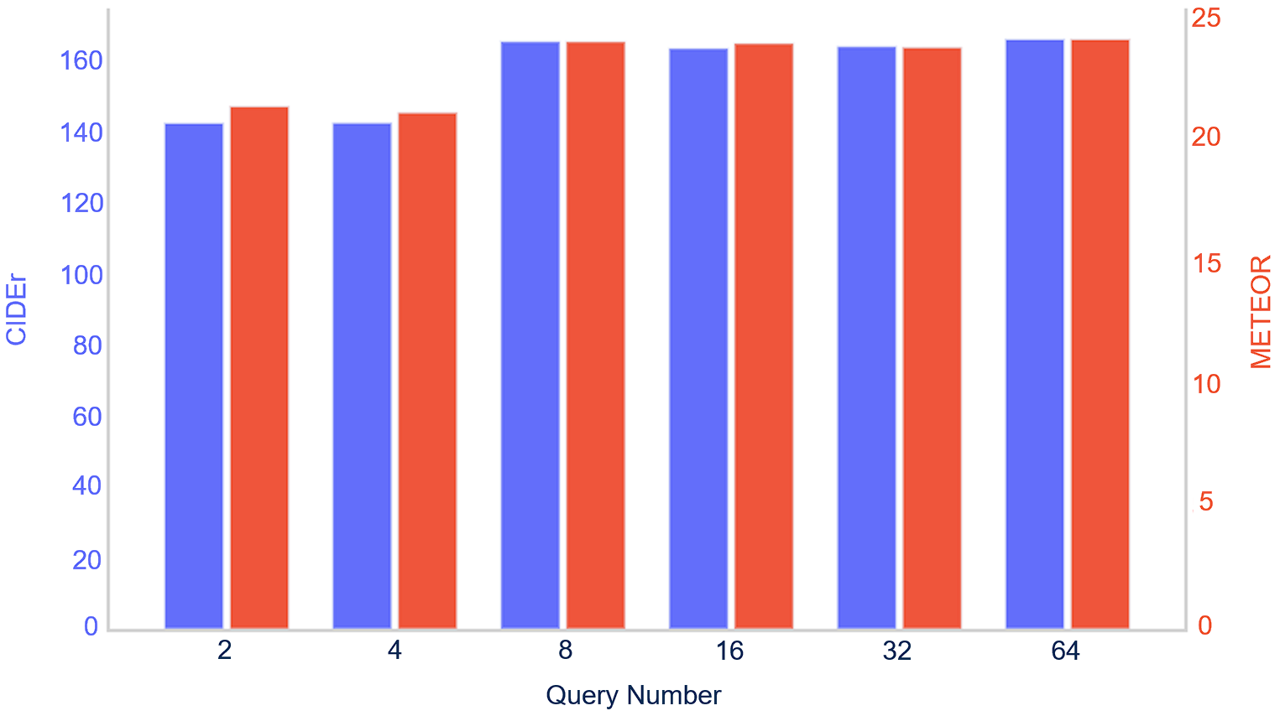
\includegraphics[width=0.4\textwidth]{fig/qnumber1.png}}
  \caption{Impact of the query numbers on the performance. For each query number, we report CIDEr (blue) and METEOR scores (red)  over the Moments-OVRE test set. }
   \label{fig:abl_qnumber}
   %removedVspace
\end{figure}


%\afterpage{%
\begin{figure*}[ht]
  \centering
  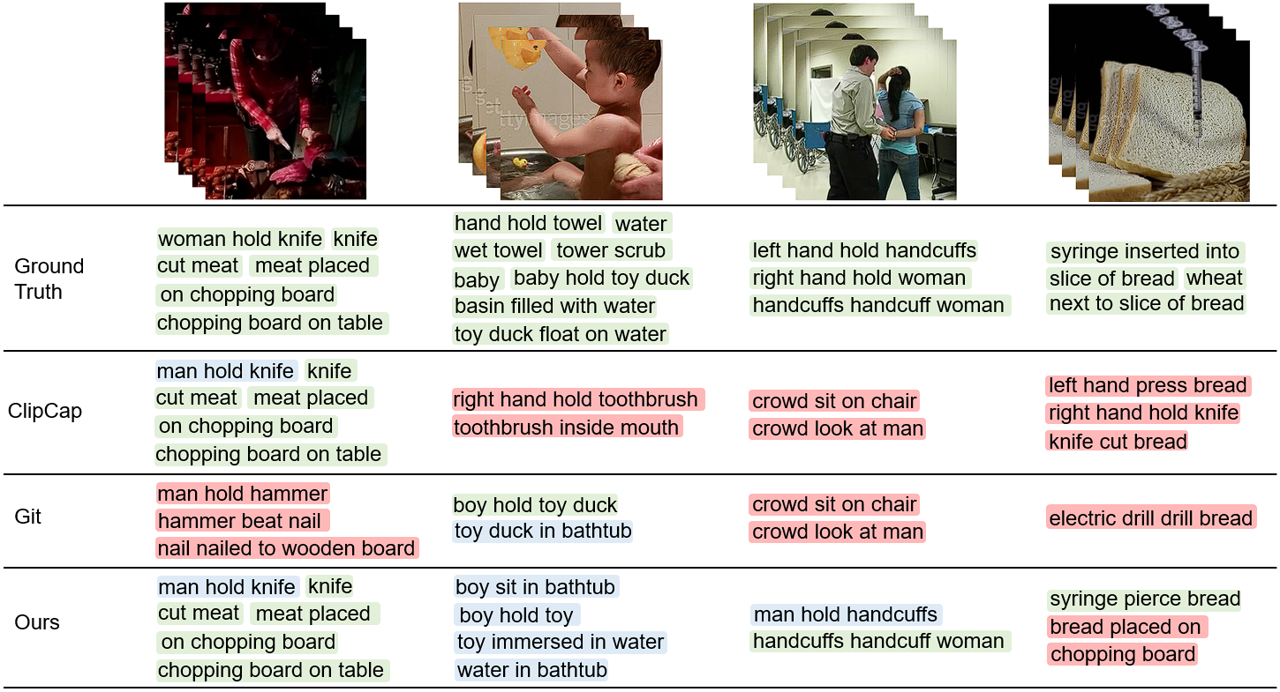
\includegraphics[width=0.9\textwidth]{fig/tab.png}
  \caption{Comparisons of triplets generation across diverse OVRE methods.
  %Correct triplets are highlighted with green backgrounds, semantically related triplets with blue backgrounds, and wrong triplets with red backgrounds.
  The illustration highlights accurately described triplets in green, triplets with semantic correlation in blue, and irrelevant triplets in red.
  }
  \label{fig:visualize}
  %removedVspace
\end{figure*}
%}

\subsection{Ablation Study}
\noindent \textbf{The Impact of Query Numbers. }
We first investigate the impact of query numbers.
Specifically, we experiment with query number=2, 4, 8, 16, 32, and 64.
Figure~\ref{fig:abl_qnumber} shows that an extremely small number of queries will yield inferior generation results since the limited queries are insufficient to extract the content in video patches.
 As the number grows from 2 to 8, the generated results show significant improvement.
 Subsequently, when the number of queries continues to double, the performance of the model gradually becomes saturated. We choose query number=64 as it demonstrated the best performance across all metrics.

\noindent \textbf{Exploration of Vision and Language Model Fine-tuning.}
Recent research~\cite{Rasheed2023vificlip} has shown that fully fine-tuned CLIP can effectively bridge the modality gap in the video domain.
As shown in Table~\ref{tab:abl_ft}, though the trainable parameters increased, fine-tuning the CLIP-ViT can improve the CIDEr score by 8.8.
% We also explore the effects of fine-tuning the text decoder.
% We observe that freezing GPT-2 would cause a significant drop in the CIDEr score.
% We believe this is because GPT-2 itself only has the ability to generate natural language, so fine-tuning is necessary to enable it to generate different forms of text.
Additionally, we delve into the outcomes of fine-tuning the text decoder. Experiments reveal that keeping GPT-2's parameters fixed results in a notable reduction in the CIDEr score. We attribute this decline to that GPT-2 is primarily proficient in generating natural language rather than triplets. Therefore, fine-tuning becomes imperative to enhance its capacity for producing rarely seen triplet sequences.
% \noindent \textbf{The Impact of Triplets' Orders. }
% Since relations in OVRE are unordered, we first investigate the impact of triplet orders.
% Specifically, we use Triplets Linearization proposed in REBEL \cite{huguet-cabot-navigli-2021-rebel-relation} to sort the subjects and predicates according to their occurrence frequency in the dataset.
% In Table x, we explored this sorting strategy.
% The results demonstrate that the order of relation triplets does not contribute to generation.
% \begin{table}[t]
%     \centering
%     \begin{tabular}{cccccc}
%         \toprule
%          Sort & B@1 & B@2 & B@3 & C & M\\
%         \midrule
%          \ding{51} & xx & xx & xx & xx & xx \\
%          \ding{55} & xx & xx & xx & xx & xx \\
%         \bottomrule
%         \\
%     \end{tabular}
%     \caption{The impact of triplets' order. \ding{51} indicates using Triplet Linearization as the sorting strategy.}
%     \label{tab:ablation1}
% \end{table}

\noindent \textbf{The Effect of Different Visual Features.}
% We conduct experiments by ablating on different granularity of visual features.
% In our proposed methods, we use patch features extracted from queries as prefixes for GPT-2.
% We also explore two  alternative representations as the input of attentional pooler;
% (i) Frame features: We directly utilize the features extracted from each individual frame using CLIP and concatenate them together to represent the frame-level features.
% (ii) Region features: Following the common practice in VidVRD, we extract a
% sequence of objects and subsequently employ a tracking algorithm to obtain a series of tracklet features. These features are then used as input to the model instead of patch features.
% Specifically, we use RegionCLIP \cite{zhong2021regionclip} pre-trained from LVIS to crop bounding box and seqNMS \cite{han2016seqnms} to perform object tracking.
Our experimental investigations involve ablations on different granularity of visual features. Within our proposed framework, we employ patch features extracted from videos as prefixes for the text decoder. Furthermore, we explore two alternative representations as inputs to the attentional pooler:
(\Rmnum{1}) Region features: Following the common VidVRD practice, we extract a sequence of objects and subsequently employ a tracking algorithm to obtain 5 tracklet features per video. These features replace patch features as input to the model. Specifically, we utilize RegionCLIP \cite{zhong2021regionclip} pre-trained from LVIS to crop bounding boxes and seqNMS \cite{han2016seqnms} for object tracking.
(\Rmnum{2}) Frame features: We directly utilize features extracted from individual frames using CLIP, concatenating them to form a representation of frame-level features.
% As shown in Table~\ref{tab:abl_feat}, both frame features and region features perform poorly.
% Naturally, the frame feature reflects the overall visual content of an image and fails to pay attention to fine-grained parts such as objects as well as relationships in it.
% To our surprise, region features perform even worse compared to frame features. We speculate that this is due to the insufficient generalization ability of existing object detectors. The diversity of object categories makes it challenging for them to accurately detect objects in our Moment-OVRE.
As depicted in Table~\ref{tab:abl_feat}, both frame features and region features exhibit poor performance. Notably, frame features capture the overall visual content of an image but overlook finer details such as objects and relationships. Surprisingly, region features fare even worse compared to frame features. We hypothesize that this is attributed to the limited generalization capability of existing object detectors. The diverse range of object categories complicates their accurate detection within our Moments-OVRE context.

% \noindent \textbf{More Evaluation with Different Backbones}


\section{Conclusion}
In this paper, we introduce a new task named OVRE, where the model is required to generate all relationship triplets associated with the video actions. Concurrently, we present the corresponding Moments-OVRE dataset, which encompasses a diverse set of videos along with annotated relationships. We conduct extensive experiments on Moments-OVRE and demonstrated the superiority of our proposed approach over other baseline methods. We hope that our task and dataset will inspire more intricate and generalizable research in the realm of video understanding.

\hspace*{\fill}

%\section{Limitation}
\noindent \textbf{Limitations:}
%Due to the high cost of annotating BBoXs, we haven't included object bounding boxes currently. We will continue building up this dataset and add BBox annotation in the further version of Moments-OVRE.
%i) We have currently omitted BBox annotation due to the high cost of annotation. However, we are committed to progressively enhancing this dataset and intend to introduce BBox annotations in upcoming versions of Moments-OVRE.
%Regarding VAU as a description task, we ignore the scene graph structure in the proposed method.
(\Rmnum{1}) This version of Moment-OVRE has currently omitted BBox annotation due to the high cost of annotation. We are committed to progressively enhancing this dataset and intend to introduce BBox annotations in upcoming versions of Moments-OVRE.
%ii) Considering OVRE as a descriptive task, we haven't considered the scene graph structure nature of Moment-OVRE in the proposed approach.
%Giving each object a personal identification as a special token is a feasible solution to solve this problem, we leave this to the community for further exploration.
%A viable resolution to address this issue is assigning a distinct token for individual object identification, and we defer this aspect to the broader research community for additional exploration.
%\wz{(\Rmnum{2}) To extract action-centric relations, learning the commonsense among action category and relations~\cite{yang2018commonsense} or implicit knowledge-driven representation learning methods~\cite{li2023knowledge, li2018deep} are promising approaches.}
(\Rmnum{2}) For extracting action-centric relations, leveraging commonsense among action categories and relations~\cite{yang2018commonsense} or implicit knowledge-driven representation learning methods~\cite{li2023knowledge, li2018deep} have shown promise. We will consider these knowledge-driven methods in future work.

\hspace*{\fill}

\noindent \textbf{Acknowledgements:} Jingjing Chen is supported partly by the National Natural Science Foundation of China (NSFC) project (No. 62072116). Zheng Wang is supported partly by the NSFC project (No. 62302453). Lechao Cheng is supported partly by the NSFC project (No. 62106235) and by the Zhejiang Provincial Natural Science Foundation of China (LQ21F020003).


 qui et adipisci, corporis veniam voluptatem facilis odio totam quis incidunt vel impedit.Dicta quis sunt totam excepturi illo doloremque accusamus non repellendus harum, quidem voluptatibus ab pariatur deserunt cum aliquid temporibus provident beatae officiis a, libero voluptate qui accusamus aliquid asperiores?Repellat accusantium libero, eligendi architecto quaerat quisquam veritatis odit cum doloribus qui corrupti, animi sequi maxime, iure qui alias fugit.Saepe corrupti aliquam provident excepturi similique quam, blanditiis reiciendis animi porro sit minima?Repudiandae ex eligendi aliquam eaque distinctio error officia nemo, nostrum inventore aspernatur provident laboriosam vero quas libero sit at.Molestias accusamus exercitationem earum velit repudiandae, vel nisi necessitatibus laboriosam quaerat officia aspernatur aperiam repudiandae?Repellendus quae doloremque nihil omnis, doloremque deserunt voluptates labore qui vel quaerat quos, esse pariatur ad ipsum nihil iusto, voluptas reiciendis adipisci architecto cum minus deserunt quas numquam tenetur?\clearpage
\bibliography{aaai24}
%\bibliographystyle{aaai}

\end{document}